%% ICSOFT 2026 -- Abstracts Track
%% Template: SCITEPRESS (SCITEPRESS.sty, article.cls, apalike.sty/bst in this dir)
%%
%% Status: English draft for co-author review
%% Source: docs/ICSOFT_2026_ABSTRACT.md


\documentclass[a4paper,twoside]{article}

\usepackage{epsfig}
\usepackage{graphicx}
\usepackage{subcaption}
\usepackage{amssymb}
\usepackage{amsmath}
\usepackage{amsthm}
\usepackage{multicol}
\usepackage{pslatex}
\usepackage{apalike}
\usepackage{caption}
\usepackage{url}
\usepackage{listings}
\usepackage{float}
\usepackage[ruled]{algorithm2e}
\usepackage{SCITEPRESS}
\usepackage[utf8]{inputenc}
\usepackage[T1]{fontenc}

\captionsetup{font=small}

\lstdefinestyle{appendixjava}{
  language=Java,
  basicstyle=\scriptsize\ttfamily,
  numbers=left,
  numberstyle=\tiny,
  stepnumber=1,
  numbersep=6pt,
  breaklines=true,
  breakatwhitespace=false,
  columns=fullflexible,
  keepspaces=true,
  showstringspaces=false,
  tabsize=4,
  frame=single,
  literate={→}{{$\rightarrow$}}1
           {↔}{{$\leftrightarrow$}}1
           {—}{{---}}1
           {Σ}{{$\Sigma$}}1
           {−}{{$-$}}1
}

%% ---------------------------------------------------------------
\title{Computing Consistent Levels for Layered Software Architecture Visualizations
       \subtitle{Separating Class Order, Package Order and Local Layout}}

\author{
  \authorname{Johannes Weigend}
  \affiliation{Weigend AM GmbH \& Co.KG, Germany/Brazil}
  \email{johannes.weigend@weigend.de}
}

\keywords{software architecture visualization, layout invariants,
  layered architecture visualization, strongly connected components,
  dependency analysis, software engineering tools}

\abstract{Layered architecture visualizations communicate dependency structure
by means of vertical positioning: elements that depend on others sit higher,
foundational elements sit lower. To be of practical value their upward edges
should either give real architectural feedback or indicate exposed cuts.
However, in many visualizations upward edges are layout artifacts rather than
findings --- drawings that can look plausible but mislead the viewer.
\par\smallskip
Levelized dependency maps are not new. Structure101's Levelized Structure Map
arranges elements into rows. Published
descriptions specify the intended visual behaviour but not the concrete
level-computation algorithm or its consistency conditions, leaving it unclear
whether an upward edge is a finding, a tolerated cycle cut, or an
implementation defect.
\par\smallskip
In this paper, we present the level computation pipeline implemented in S202, an
open-source Java architecture-visualization tool under
Apache~2.0.\protect\footnote{\protect\url{https://github.com/jweigend/S202}}
The pipeline has four phases, executed in a single forward pass. First,
S202 detects global SCCs in the class graph and heuristically cuts large
cycles. Second, from weighted package dependencies it derives an
architectural hypothesis: more heavily used packages sit lower, their
users higher. Third, it computes a local level per parent container that
determines vertical placement of siblings. Fourth, a horizontal-ordering
pass shortens arrows without touching levels or invariants.
\par\smallskip
The algorithmic contribution is the strict separation of architectural
hypothesis from layout position. Package analysis decides which package
directions are normal, cyclic, or heuristically cut; local placement only
decides where classes and visible containers appear inside one concrete parent.
This prevents feedback loops in which class feedback, package order, and local
positions redefine each other.
\par\smallskip
Five machine-checkable invariants act as implausibility alerts to the
developer: class dependencies respect class levels after heuristic cuts, dominant
weighted package dependencies respect package levels, cyclic peer packages
share a level after filtering, visual ranks follow local levels, and
cached edge classifications match the current SCC and level state. Four of these
alerts are pipeline-defect detectors that never fire on a correct run; the
fifth fires only on remaining upward edges from broken cycles and points to a
concrete architecture violation. On an acyclic codebase, S202 therefore
produces an alert-free layout in which every edge points downward.
\par\smallskip
We demonstrate the pipeline on Minecraft Forge~1.19.2, a large and highly
cyclic system that stresses every stage. Separating global architecture depth
from local layout, and preserving the computed package order in the UI
instead of reordering it to suppress cycles, reduces the visual upward-edge
count from roughly~6\,000 to~4\,157; the remaining edges are real
architecture violations or explicit heuristic cuts.
\par\smallskip
The result is a reproducible level-computation algorithm: every visible
anomaly is a finding, not an artifact.}
%% ---------------------------------------------------------------

\begin{document}

\maketitle

\begin{center}
  \fbox{\textbf{\large Draft Version 4 \quad|\quad \today}}
\end{center}

\vfill

\bibliographystyle{apalike}
{\small
\bibliography{icsoft2026_EN}}

%% ===================================================================
\appendix
\onecolumn

\section*{Appendix A -- Algorithm in Detail}

This supplementary material expands the one-page abstract.

\subsection*{Bird's-eye view}

The pipeline is a single forward pass through four deterministic
phases. There is no iteration, no fixed-point loop, no search for a
minimum-violation arrangement, and no resorting after the fact.

\begin{itemize}\setlength{\itemsep}{2pt}
  \item \textbf{Phase 1 --- Class order.}
        Collapse the class dependency graph into SCCs, break large
        SCCs by a degree-rank heuristic, then assign every class an
        \emph{architecture level} by longest path on the SCC-DAG.
        Feeds the tangle view, the SCC display, and the class-level
        invariant check; does not drive the 2D ($x,y$) layout, but
        the class architecture level can be mapped to $z$ in 3D views
        as a complexity-height encoding.
  \item \textbf{Phase 2 --- Package order.}
        On the weighted inter-package graph, break SCCs by a weight-rank
        heuristic, then assign every package an \emph{architecture
        level}. Feeds the package-level invariant checks and is
        consumed by Phase 3 as a hard constraint.
  \item \textbf{Phase 3 --- Place classes into the package frame.}
        Phase 2 has fixed the vertical order of packages; Phase 3
        leaves that order intact and only places the classes within
        each parent. For each parent container, it builds the
        sibling-only graph from class-call counts, breaks any local
        cycles by first cutting edges that contradict the package
        architecture (so Phase 2's order is never touched), and
        assigns each class a \emph{local level} by longest path on
        the SCC-DAG. Sub-package siblings keep the order Phase 2
        gave them; only classes are newly positioned.
  \item \textbf{Phase 4 --- Horizontal arrangement.}
        Within each row, place siblings horizontally so inter-sibling
        arrows are short and rarely cross. Does not change any level
        and is deliberately excluded from the layout invariants.
\end{itemize}

Figure~\ref{fig:s202-deps-overview} shows the result of Phases~1--4 on
two example projects: an acyclic test JAR (left) and a cyclic real-world
subsystem (right). The next paragraph explains what the arrows in those
panels mean; the paragraph after that explains how the invariants relate
to them.

\begin{figure}[H]
  \centering
  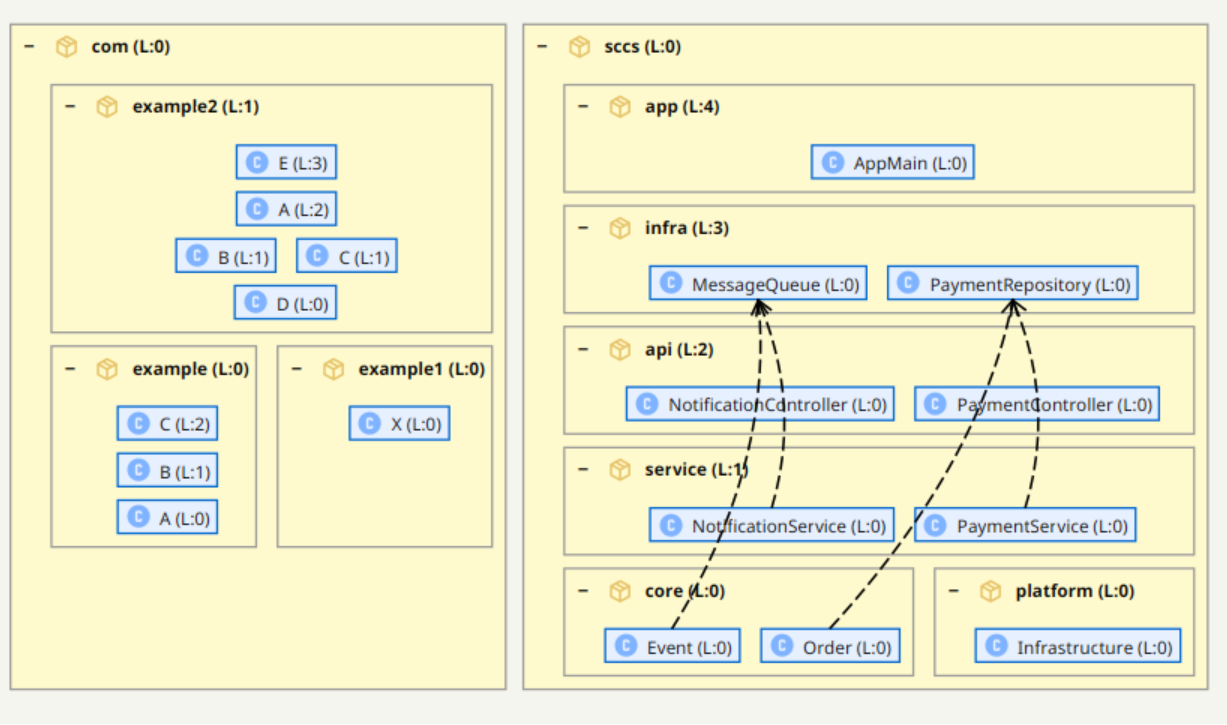
\includegraphics[width=0.95\textwidth]{figures/S202-Dependencies.png}
  \caption{The S202 ArchitectureView with class and package boxes.
    \textbf{Left:} an acyclic situation taken from the test JAR
    (\texttt{com.example.\ldots}) --- no upward edges, no alerts; the
    downward \texttt{NORMAL} arrows that are normally suppressed have
    been turned on here to make the layered structure visible.
    \textbf{Right:} a real-world cycle between \texttt{core}, \texttt{infra}
    and \texttt{service}; the remaining upward edges trigger R1-visual
    alerts that flag concrete architecture violations.}
  \label{fig:s202-deps-overview}
\end{figure}

\paragraph{Where the arrows come from.} The arrows visible in
Figure~\ref{fig:s202-deps-overview} are not produced by the four pipeline
phases. They are the class-to-class dependencies extracted from the
bytecode in the very first analysis step, long before any level is
computed. Phases~1--4 decide \emph{where the boxes go}; the renderer then
simply draws an arrow from each source box to each target box. By default
the renderer suppresses downward \texttt{NORMAL} arrows, so the eye is
drawn to upward edges and explicit cuts; the left panel of
Figure~\ref{fig:s202-deps-overview} has that toggle turned on, which is
why every downward dependency is visible there. The renderer distinguishes
three arrow classes (\texttt{EdgeType} in the code):
\begin{itemize}\setlength{\itemsep}{1pt}
  \item \texttt{NORMAL} -- source box ends up above target box (thin solid
        downward arrow; hidden in the default view, visible in the left
        panel of Figure~\ref{fig:s202-deps-overview});
  \item \texttt{VIOLATION} -- source box ends up below target box (upward
        arrow, drawn dashed and bold; visible by default);
  \item \texttt{INTRA\_SCC} -- both endpoints sit in the same cyclic group
        (peer-level arrow, drawn red when the user enables the SCC overlay,
        otherwise suppressed).
\end{itemize}
After the SCC-breaker removes a back-edge to obtain a usable hierarchy, the
endpoints end up at different architecture levels in the resulting DAG; the
removed back-edge then runs against that hierarchy and the classifier
labels it as a plain \texttt{VIOLATION}. The SCC-breaker keeps its own
bookkeeping of which violations are deliberate cuts, so the invariant
checker can suppress them when judging algorithmic correctness, but the
arrow in the picture is visually indistinguishable from a real violation.
At the package level the same three classes apply, but inter-package edges
are bundled and labelled with a filled circle that carries the aggregated
call count, so the diagram does not drown in one line per class reference.

The five invariants then \emph{read} the placed boxes and the classified
arrows. They do not change either; they only check that the two agree
with the architecture data and with each other. Concretely, R1-algo and
R1-visual check the agreement between an arrow's direction and its
endpoints' levels; R2 and R3 check the package-level placement; R5
checks that the cached arrow classification still matches the current
levels.

\paragraph{Invariants act as implausibility alerts.} The invariants run
\emph{after} the pipeline (R is short for \emph{rule}; the catalogue
contains R1--R5, with R4 retired and absorbed into R2, see
Section~``R4: A Retired Rule''). They are not a feedback signal that
drives further iteration. Four of them (R1-algo, R2, R3, R5) are
pipeline-defect alerts that never fire on a correct run; the fifth
(R1-visual) fires when a remaining upward arrow points to a real
architecture violation. Every visible upward arrow in the resulting
drawing is therefore either a \texttt{VIOLATION} (raising an R1-visual
alert -- which is further divided in the SCC-breaker's bookkeeping into
a real architectural finding or a deliberate heuristic cut) or, when the
SCC overlay is on, an \texttt{INTRA\_SCC} edge that could not be broken
without contradicting the package architecture --- never an accidental
artifact of the layout algorithm.

\begin{figure}[H]
  \centering
  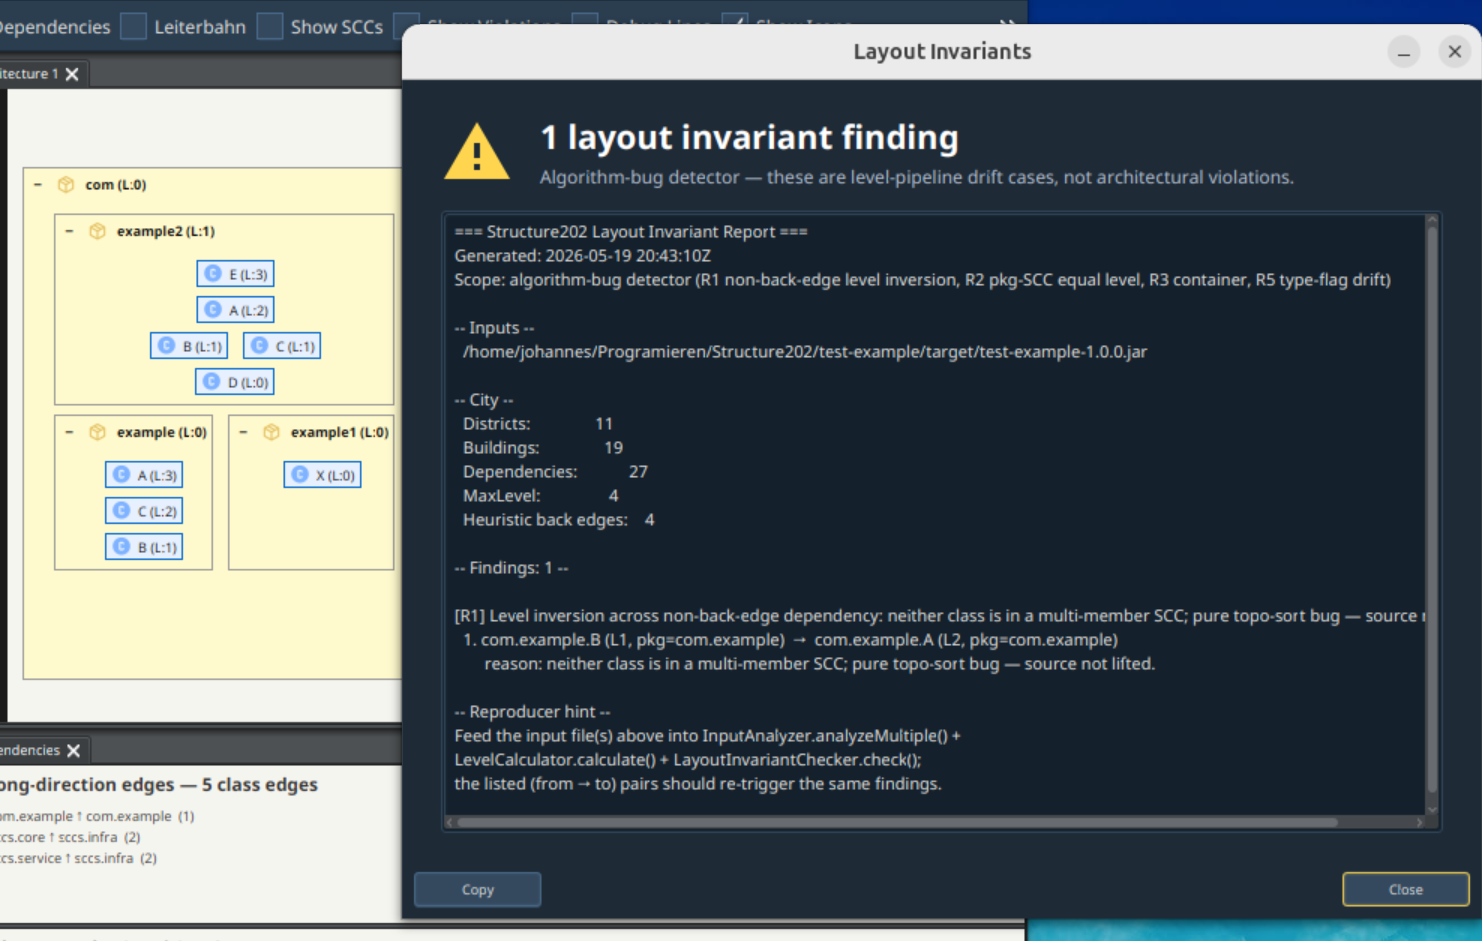
\includegraphics[width=0.95\textwidth]{figures/Finding-R1-Wrong-Direction.png}
  \caption{Implausibility alert in action. For this screenshot we deliberately
    injected a level-pipeline defect into \texttt{LevelCalculator} that
    misplaces class \texttt{com.example.A} on the wrong level (compare with
    Figure~\ref{fig:s202-deps-overview}, left, which shows the correct
    placement of the same test JAR). The post-pipeline invariant checker
    catches the inconsistency immediately and pops up the
    \emph{Layout Invariants} dialog: a single R1 finding with a copy-paste
    reproducer block tells the developer that the dependency
    \texttt{B}~$\rightarrow$~\texttt{A} now runs against the computed levels.
    The status bar additionally reports the four wrong-direction class edges
    induced by the bug. No human inspection of the picture was needed to
    surface the defect; the alert is generated automatically by the
    invariant checks that run after every analysis.}
  \label{fig:r1-wrong-direction}
\end{figure}

The dialog text in Figure~\ref{fig:r1-wrong-direction} is small at print
size, so the same report is reproduced verbatim below as it appears in the
log and the dialog:

\begin{lstlisting}[basicstyle=\scriptsize\ttfamily,frame=single,breaklines=true,columns=fullflexible,xleftmargin=0pt,xrightmargin=0pt]
16:43:05.166 [JavaFX Application Thread] WARN de.weigend.s202.ui.wfx.S202Module
-- Layout invariant report (1 finding(s)):
=== Structure202 Layout Invariant Report ===
Generated: 2026-05-19 19:43:05Z
Scope: algorithm-bug detector (R1 non-back-edge level inversion,
       R2 pkg-SCC equal level, R3 container, R5 type-flag drift)

-- Inputs --
  /home/johannes/Programieren/Structure202/test-example/target/test-example-1.0.0.jar

-- City --
  Districts:               11
  Buildings:               19
  Dependencies:            27
  MaxLevel:                 4
  Heuristic back edges:     4

-- Findings: 1 --

[R1] Level inversion across non-back-edge dependency: neither class is
     in a multi-member SCC; pure topo-sort bug -- source not lifted.
  1. com.example.B (L1, pkg=com.example)  ->  com.example.A (L2, pkg=com.example)
       reason: neither class is in a multi-member SCC;
               pure topo-sort bug -- source not lifted.

-- Reproducer hint --
Feed the input file(s) above into InputAnalyzer.analyzeMultiple() +
LevelCalculator.calculate() + LayoutInvariantChecker.check();
the listed (from -> to) pairs should re-trigger the same findings.
\end{lstlisting}

The remainder of this appendix walks through the algorithm in detail:
the core problem and four failure modes that motivate the
three-coordinate model, the solution, the layout invariants, the
complete pipeline, the \emph{software-ekg-7} fix that the invariant
checker caught, a summary, and a Q\&A section.
Appendix~B contains the reference implementation.

\subsection*{The Core Problem: Architectural Hypothesis, Local Layout, Five Consistency Checks}

A correct layered layout has to separate an architectural hypothesis from the
local placement that makes this hypothesis visible. In S202 this means answering
three related questions that are often treated as one ordering problem:

\begin{itemize}
  \item \emph{Class analysis} -- where does a class sit in the global class
        dependency stack? This is the longest-path depth in the
        SCC-collapsed class graph.
  \item \emph{Package analysis} -- what package order is implied by the
        aggregated dependency traffic? This architectural hypothesis is
        computed on the weighted inter-package graph, independently of the
        deepest contained class.
  \item \emph{Local layout} -- where should an element's box sit inside its
        parent container? Only dependencies between classes in the subtrees of
        that parent's direct children decide this local level.
\end{itemize}

The three computed values are independent in principle, and the implementation
must keep the package-level hypothesis separate from local layout choices.
Mixing them is the root cause of every failure mode below. Five consistency
checks then inspect the resulting levels and rendered order:

\begin{enumerate}
  \item \textbf{Class-level consistency (R1-algo):} If
        $A \rightarrow B$ denotes a class dependency, then
        $\text{archLvl}(A) > \text{archLvl}(B)$ after heuristic back-edges are
        removed. This checks the longest-path assignment in the
        class-dependency SCC-DAG.
  \item \textbf{Visual-rank consistency (R1-visual):} For every class
        dependency $A \rightarrow B$ that is not a heuristic back-edge, the
        rendered position of $A$ in its parent box chain sits above $B$. The
        comparison is lexicographic on the tuple of local levels along
        the parent path, ending with the class's own local level. This is the
        statement represented by the drawing.
  \item \textbf{Package-SCC consistency (R2):} Packages that form a cyclic
        group in the filtered package dependency graph share the same package
        architecture level.
  \item \textbf{Package-order consistency (R3):} In the weighted inter-package
        dependency graph, when the call traffic from package $P_A$ to $P_B$
        dominates the reverse, $P_A$ ends up at a strictly higher package
        architecture level than $P_B$.
  \item \textbf{Classification consistency (R5):} Cached edge classifications
        such as \texttt{NORMAL}, \texttt{VIOLATION}, and \texttt{INTRA\_SCC}
        match the current level assignment and SCC membership.
\end{enumerate}

R1-algo, R2, R3 and R5 check the algorithmic model; R1-visual checks the
rendered order. The failure modes that follow show why each obvious shortcut
collapses one of these concerns into another and loses information.

\subsection*{Relation to Structure101 and Levelized Structure Maps}

Structure101's Levelized Structure Maps are a closely related practical
predecessor to the layout studied here. They organize code elements into rows
such that, as far as possible, dependencies flow downward, and they expose
feedback dependencies when cyclic regions prevent strict
levelization~\cite{HeadwayLSM,HeadwayMatrix}. This makes Structure101 an
important point of comparison and a necessary part of the related work.

The public Structure101 documentation, however, describes the intended
properties of the visualization rather than the concrete algorithm that computes
the rows. The same is true for academic references that discuss Structure101 as
a software architecture analysis tool or as related work for layered
visualization~\cite{Muccini2012}: they characterize the LSM concept, but do not
provide an algorithmic specification of Structure101's levelization procedure.
To the best of our knowledge, no published paper describes the exact
Structure101 algorithm.

S202 therefore provides an open algorithmic account of a related class of
levelized dependency layouts, not a claim that the visual idiom itself is new.
The novelty lies in making the computation explicit, separating class
architecture depth, package architecture order, and local layout position, and
checking the resulting layout through executable invariants.

S202 also continues a line of work the author has co-published on layered
dependency visualization. \cite{Dashuber2021} introduced a layered software-city
metaphor that uses building height for architectural depth, and \cite{Dashuber2022}
extended it with static and dynamic dependency overlays. Both papers describe
the visual idiom and the supporting infrastructure but treat the underlying
level computation as a single coordinate; they do not separate class
architecture depth, package architecture order, and local layout position, and
they do not introduce machine-checkable invariants. The present paper closes
this algorithmic gap for the 2D layered view in S202.

\subsection*{Failure Mode 1: Cascading Level Updates}

An algorithm iterates over classes and assigns levels. It first sees class $A$
in package $P_1$, computes $\text{level}(A)=3$, and therefore sets
$\text{level}(P_1)=3$. Later it reaches class $B$ in package $P_2$ and
discovers that $A$ and $B$ are in the same SCC and must share a level, now
$\text{level}(A)=\text{level}(B)=5$. This forces $P_1$ to be recomputed. If
$P_1$ depends on $P_3$, $P_3$ may need to move as well. A cascade follows.

In a naive single-pass implementation, however, $P_1$ and $P_3$ may already have
been finalized. SCC membership is only known after the relevant graph has been
traversed; if level assignment and SCC discovery are interleaved, the iteration
order decides whether the correction is still applied in time.

\subsection*{Failure Mode 2: Interleaved Cycle Detection Produces
Classpath-Dependent Results}

The most subtle practical failure mode occurs when cycle detection and level
computation are not separated. The algorithm traverses the class graph, assigns
levels, and handles discovered cycles on the fly, depending on which class
happens to be processed first.

Classes come from JARs. The order in which the JVM sees classes follows the
order in which they were packaged into the JAR. That order can depend on the
build tool, module order in a multi-module build, filesystem ordering on the
build server, and other implementation details. None of these orders is
semantically meaningful; none encodes architectural dependency direction.

The result is unreliable: the same source code can produce different level
layouts under different build configurations. The errors are subtle. The layout
may still look plausible, arrows may mostly point in the expected direction,
and no obvious visual break appears. Yet the precise hierarchy information is
corrupted and may remain unnoticed for a long time.

The solution is to separate the phases strictly: first compute the SCC
partition on the complete graph, then build the SCC-DAG, then assign levels.
Tarjan's algorithm computes the SCC partition in $O(V+E)$; with deterministic
input ordering, the implementation becomes reproducible and independent of
classpath traversal artifacts.

\subsection*{Formal Counterexample: Why a Naive Recursive Algorithm Fails}

The intuitive level-computation algorithm is a recursive DFS with memoization:

\begin{verbatim}
level(A):
  if A already computed: return level(A)
  if A has no dependencies: return 0
  return max(level(dep) for dep in A.dependencies) + 1
\end{verbatim}

For acyclic graphs this is correct and equivalent to longest-path computation
on a DAG. For cyclic graphs it fails structurally.

\textbf{Counterexample with two SCCs:}

\begin{verbatim}
SCC_1 = {A, B}, with A -> B -> A
SCC_2 = {C, D}, with C -> D -> C
Cross dependency: A -> C
\end{verbatim}

The correct levels are $\text{level}(C)=\text{level}(D)=0$ and
$\text{level}(A)=\text{level}(B)=1$.

Recursive algorithm, starting at $A$:

\begin{verbatim}
level(A)  [A "in progress", sentinel = 0]
  -> level(B)
      -> level(A): cycle detected, return 0
    B.level = 0 + 1 = 1
  -> level(C)  [C "in progress", sentinel = 0]
      -> level(D)
          -> level(C): cycle detected, return 0
        D.level = 0 + 1 = 1
    C.level = 1 + 1 = 2   <-- wrong; correct would be 0
  A.level = max(1, 2) + 1 = 3   <-- wrong; correct would be 1
\end{verbatim}

After SCC equalization, $\text{SCC}_1=\max(3,1)=3$ and
$\text{SCC}_2=\max(2,1)=2$. Both results are wrong.

The cause is that the recursive algorithm enters $\text{SCC}_2$ from the
context of $\text{SCC}_1$. The sentinel-based local cycle handling inflates the
level of $\text{SCC}_2$, and that inflated level then feeds into the
computation of $\text{SCC}_1$. The correct level of $\text{SCC}_2$, namely
zero, is only known after the graph has been collapsed into SCCs and evaluated
as an SCC-DAG.

Thus, recursive level algorithms that mix traversal, cycle handling, and level
assignment can produce traversal-order-dependent results on graphs with
interacting SCCs. In JVM-based tools, that traversal order can be influenced by
classpath and packaging order. The correct solution collapses SCCs before level
assignment: Tarjan, then SCC-DAG, then longest path.

\subsection*{Failure Mode 3: Deriving Package Levels from Class Levels}

An obvious implementation assigns each package a level equal to the maximum
level of its contained classes, then lifts parent packages transitively.
This is wrong for two reasons.

First, the rule conflates containment with dependency. A package that
\emph{contains} a class at level~7 is not necessarily architecturally
positioned at level~7 itself; it may have no cross-package dependencies
at all. Two disconnected package trees processed from the same JAR would
be ordered relative to each other by accident of their class contents,
not by their actual dependency relationships.

Second, the approach creates a circular dependency between the two
level systems: class levels depend on the class graph, but package levels
derived from class levels then constrain the visual position of packages
relative to classes, making the combined coordinate system ill-defined.

S202 avoids this by computing class levels and package levels on
independent graphs with no mutual constraint. Each system starts at zero and
grows according to its own dependency structure.

\subsection*{Failure Mode 4: Large SCCs Without Heuristics Collapse
the Layout}

Without a mechanism for breaking large SCCs, all members of a cyclic group must
be placed on the same level. For small cycles of two to five classes this is
acceptable. For Minecraft Forge~1.19.2 (5\,123 classes), however, we observed a single
SCC containing 2\,857 classes. Without a breaker, more than 55~percent of the
project would be assigned the same level. All remaining classes would be
distributed above, but the internal dependency hierarchy within this large
cycle would be invisible.

The heuristic SCC breaker solves this practical problem. It identifies back
edges---dependencies that run against the inferred architecture direction---and
removes them for level computation. The removed edges are visualized as
violations instead of being ignored. The layout preserves visibility of
cyclic dependencies while still producing a usable hierarchy.

\subsection*{Relation to Feedback Arc Set Heuristics}

Failure Mode 4 is an instance of the Minimum Feedback Arc Set problem: remove a
minimal set of directed edges so the graph becomes acyclic. The problem is
NP-hard \cite{Karp1972}, so any practical polynomial-time implementation must
use a heuristic or approximation.

A well-known related heuristic is due to Eades, Lin, and Smyth \cite{Eades1993}.
It orders nodes according to the difference between outgoing and incoming
degree, then classifies edges that point backward in the resulting sequence as
feedback edges. The intuition is similar to S202: high out-degree
suggests a higher-level element; high in-degree suggests a lower-level
element.

S202 uses a deliberately simpler variant: a direct normalized score per
node,

\[
  r(P) = \frac{\text{outWeight}(P) - \text{inWeight}(P)}
              {\max(1,\; \text{outWeight}(P) + \text{inWeight}(P))},
\]

where the weights are summed within the SCC under consideration. At the class
level the weights are the in- and out-degrees in the class dependency graph;
at the package level they are aggregated method-call counts. An edge
$P_A \to P_B$ inside an SCC is classified as a back-edge candidate when
$r(P_A) < r(P_B) - 0.1$. Equal-rank pairs represent symmetric bidirectional
dependencies with no dominant architectural direction; they remain in the same
SCC and are assigned the same level.

The important distinction is transparency. Many tools break cycles implicitly,
but S202 classifies heuristic cut edges explicitly. They are marked as
\texttt{VIOLATION}, rendered as a bold dashed upward arrow, and known to the
invariant checker. This
makes algorithmic defects separable from tolerated heuristic artifacts.

\subsection*{The Solution: Three Computed Values on Independent Graphs}

Failure modes 1 to 3 share a root cause: conflating values that belong to
different semantic domains. S202 resolves this by computing three independent
values, two of them for analysis and one for layout.

\begin{itemize}
  \item \textbf{Class architecture level} is the longest path in the
        SCC-collapsed class dependency DAG. It represents global architectural
        depth: how many layers of dependencies separate a class from the
        bottom of the analysed dependency graph.
  \item \textbf{Package architecture level} is the longest path in the
        SCC-collapsed weighted inter-package dependency graph. Edge weights are
        method-call counts aggregated from class-level references. The result
        represents the module's position in the system's overall dependency
        order, independently of the class-level coordinate.
  \item \textbf{Local level} is the longest path in the SCC-collapsed
        sibling-only dependency graph of a single parent container. The graph
        contains only edges whose source and target both lie in some direct
        child of that parent; references leaving the parent's subtree are excluded
        because they are handled by the enclosing container. Every
        element (class and package) gets a local level that is only
        meaningful within its own parent box. The renderer sorts each parent's
        children by this index, so the visible Y position of a box is the
        local level, not the global architecture level.
\end{itemize}

All three concepts use the same algorithmic shape---Tarjan SCC detection,
weight-based back-edge identification, DAG condensation, longest-path
propagation---but on three different graphs with three different scopes.
Because the systems are independent, packages with no cross-package
dependencies correctly land at architecture level~0 regardless of the class
levels inside them, and a top-level class like \emph{ArchitectureView} that
orchestrates a sub-package such as \emph{ui.rendering} sits visually above the
sub-package box without distorting either of their architecture levels.

The separation is an engineering choice driven by semantic clarity. A unified
single-coordinate approach is theoretically possible, but it conflates three
semantically distinct concerns---global architectural depth, module dependency
order, and per-container visual position---into one number, making the pipeline
hard to reason about, test, and maintain. Each simplification of such
a unified approach turns into one of the failure modes above.

The three concepts have the following algorithmic structure. Phases~1 and~2
compute the global architecture levels; Phase~3 derives the local level
per parent container from the architecture-level output.

\begin{algorithm}[H]
\DontPrintSemicolon
\caption{Phase~1 -- Global Class Levels (\texttt{LevelCalculator}, Step~3)}
class dependency graph\;
\Indp $\rightarrow$ Tarjan (SCCs)\;
$\rightarrow$ SCCBreaker: identify heuristic back-edges in large SCCs ($|S| \geq 3$; 2-class SCCs are equalized instead)\;
\hspace{1.5em} rank$(P)=(\text{outDeg}-\text{inDeg})\,/\,\max(1,\text{outDeg}+\text{inDeg})$\;
\hspace{1.5em} edge $A\!\to\!B$ is a back-edge candidate if $\text{rank}(A)<\text{rank}(B)-0.1$\;
$\rightarrow$ Remove back-edges $\rightarrow$ filtered class DAG\;
$\rightarrow$ Condense into SCC-DAG $\rightarrow$ longest-path pass\;
$\rightarrow$ Assign SCC level to all member classes (equalization implicit)\;\Indm
\end{algorithm}

\begin{algorithm}[H]
\DontPrintSemicolon
\caption{Phase~2 -- Package Architecture Levels (\texttt{LevelCalculator}, Step~4)}
\textbf{Build weighted inter-package dependency graph} $G_P=(V_P,E_P,w)$:\;
\Indp
  For each class $C$ in package $P_\text{leaf}$ with method calls to class $D$ in $P_\text{target}$ ($P_\text{leaf} \ne P_\text{target}$):\;
  \hspace{1em} $w(P_\text{ancestor},\, P_\text{target})\ \mathrel{+}=\ \text{callCount}(C \to D)$\;
  \hspace{1em} for every ancestor $P_\text{ancestor}$ of $P_\text{leaf}$ with $P_\text{ancestor} \ne P_\text{target}$\;
  Fallback weight $= 1$ for structural references with no method-call data\;
  No directional filtering: both parent$\to$child and child$\to$ancestor edges enter $G_P$. The SCC breaker decides direction by weight.\;
\Indm
\BlankLine
\textbf{Iterative SCC-breaking} (repeat until stable):\;
\Indp
  Tarjan on current graph $\rightarrow$ find SCCs with $|S|\ge 2$ (2-package SCCs broken if rank differs; equalized otherwise)\;\;
  For each member $P \in S$:\;
  \hspace{1em} $r(P) = \bigl(\sum_{Q\in S}w(P,Q)-\sum_{Q\in S}w(Q,P)\bigr)\;/\;\max\!\bigl(1,\textstyle\sum_{Q\in S}w(P,Q)+\sum_{Q\in S}w(Q,P)\bigr)$\;
  Edge $P_A\!\to\!P_B$ inside $S$ is a back-edge if $r(P_A) < r(P_B) - 0.1$; remove it\;
  Equal-rank pairs remain in the SCC $\rightarrow$ assigned the same level\;
\Indm
\BlankLine
\textbf{Level assignment}:\;
\Indp
  Condense remaining graph into SCC-DAG\;
  Longest-path propagation on SCC-DAG\;
  Assign SCC level to all member packages\;
\Indm
\end{algorithm}

Phase~1 produces classpath-independent class architecture levels because SCCs
are collapsed before levels are assigned. Phase~2 produces package architecture
levels directly from package dependencies: every class reference contributes to the weighted graph regardless of
the containment relation between source and target package, and a per-SCC
rank score decides which direction of a cyclic group dominates. The two
architecture coordinate systems do not constrain each other---a package with
no outgoing cross-package calls lands at level~0 regardless of the class
levels inside it, and conversely the class levels of a package's contents
do not lift the package itself.

\begin{algorithm}[H]
\DontPrintSemicolon
\caption{Phase~3 -- Local Level per Parent Container (\texttt{LocalLevelCalculator}, Step~6)}
\textbf{for each} parent package $P$ with at least two direct children:\;
\Indp
  Let $S(P)$ be the direct children (classes and sub-packages).\;
  Build sibling-only weighted graph $G_P^{\,\text{loc}}$ on $S(P)$:\;
  \hspace{1em} edge $X \to Y$ with weight $\textstyle\sum \text{callCount}(c \to d)$\;
  \hspace{1em} over all class refs $c \to d$ where $c$ lies in the subtree of sibling $X$\;
  \hspace{1em} and $d$ lies in the subtree of sibling $Y$;\;
  \hspace{1em} refs leaving the parent's subtree are excluded.\;
  Tarjan on $G_P^{\,\text{loc}}$ $\rightarrow$ SCCs.\;
  Within each SCC of size $\ge 2$: evaluate every candidate edge cut.\;
  First cut an edge that contradicts the package architecture; only then\;
  prefer the cut that maximally decomposes the SCC; edge weight and rank as further tie-breakers.\;
  Condense to SCC-DAG, longest-path pass, assign \textbf{localLevel} per sibling.\;
\Indm
\end{algorithm}

Phase~3 is a pure layout phase. It never modifies architecture levels. Each
parent container gets its own computation: a class's local level inside
\emph{ui} carries no relationship to a class's local level inside
\emph{ui.rendering}. The renderer sorts each parent's children by their local
level, descending. The enclosing parent's local level handles
cross-container ordering recursively. The local SCC breaker resolves local
cycles---for example, two sibling sub-packages with mutual class
references---silently. It removes one edge at a time, always preferring an
edge that contradicts the package architecture: Phase~3 may never reorder
packages relative to the order computed in Phase~2. Only when no
architecture-contradicting edge is available does the breaker fall back on
cycle-decomposition score, edge weight, and rank. S202 does
not surface these local cycles as a separate Tangle category because the
user-visible tangle list remains a global architecture statement.

After Phase~3 the level computation pipeline is finished. A fourth phase, the
horizontal-arrangement pass (\texttt{HorizontalRowLayoutOptimizer}),
runs purely for the legibility of inter-sibling dependency arrows:
it reorders same-row siblings so related elements sit horizontally
close. It modifies no level, no SCC membership, and no invariant
result, and is therefore mentioned here only for completeness; the
detailed algorithm appears later in this appendix.

\begin{table}[h]
\centering
\small
\begin{tabular}{llll}
\hline
 & \textbf{Phase 1 -- Class} & \textbf{Phase 2 -- Package} & \textbf{Phase 3 -- Local Level} \\
\hline
\textbf{Graph}        & Class dependency             & Weighted inter-package        & Sibling-only weighted (per parent) \\
\textbf{Edge weight}  & Unweighted                   & Method-call counts            & Method-call counts \\
\textbf{Scope}        & Global                       & Global                        & Per parent container \\
\textbf{Meaning}      & Class arch. depth            & Module dep. position          & Visual Y in parent box \\
\textbf{Zero point}   & Class with no deps           & Package with no outgoing calls & Bottom sibling in box \\
\textbf{Cycles}       & SCCBreaker (degree)          & Weight-rank, all edges        & Max-cycle-break within siblings \\
\textbf{Used by}      & R1-algo, Tangles             & R3, R2                        & R1-visual, renderer sort \\
\hline
\end{tabular}
\caption{The three independent values computed by S202.}
\end{table}

\subsection*{Layout Invariants for Level Correctness}

The three level phases are guarded by five machine-checkable invariants
that act as the implausibility alerts introduced in the abstract. All five
run after the pipeline as post-checks on the fully computed model and the
rendered layout; none feeds back into level assignment. In the current code
base R1-algo, R2, R3, and R5 are evaluated by the
\texttt{LayoutInvariantChecker}, while R1-visual is checked by the
architecture builder as part of its violation-detection pass over the
visual-rank tuple --- a historical split with no semantic consequence; both
halves act as identical post-checks. These checks are evidence that the
computed model is internally consistent; they are not the primary
algorithmic contribution.

\begin{table}[h]
\centering\small
\begin{tabular}{lp{10.5cm}}
\hline
\textbf{Rule} & \textbf{Consistency check} \\
\hline
R1-algo    & Non-heuristic class dependencies respect class architecture levels:
             $A \rightarrow B \Rightarrow \text{archLvl}(A) > \text{archLvl}(B)$.
             Tests the longest-path assignment of Phase~1. \\
R1-visual  & For every non-heuristic class dependency $A \rightarrow B$, the
             rendered position of $A$ sits above $B$. The check compares positions
             lexicographically on
             $\bigl[L(\text{ancestor}_1),\ldots,L(\text{ancestor}_n),\,L(A)\bigr]$
             versus $\bigl[L(\text{ancestor}_1'),\ldots,L(\text{ancestor}_m'),\,L(B)\bigr]$
             where $L$ denotes the local level. Covers same-parent,
             same-grandparent, and cross-tree comparisons uniformly. \\
R2         & Packages forming a cyclic group in the filtered package dependency
             graph share the same package architecture level. \\
R3         & For every weighted package edge $(P_A, P_B)$ with $w(P_A,P_B) > w(P_B,P_A)$
             that is not a back-edge cut by the SCC breaker:
             $\text{archLvl}(P_A) > \text{archLvl}(P_B)$. \\
R5         & Cached edge classifications (\texttt{NORMAL}, \texttt{VIOLATION},
             \texttt{INTRA\_SCC}) remain consistent with the current level
             assignment and SCC membership. \\
\hline
\end{tabular}
\caption{Five layout consistency checks verified after every analysis run. R1-algo,
R3 and R2 check the algorithm; R1-visual checks the rendered picture; R5
keeps the cached annotations consistent.}
\end{table}

Throughout the iterative development of the level computation pipeline, R2 surfaced
implementation bugs after algorithm changes that the unit-test suite had not
detected.
Figure~\ref{fig:invariant-r2} shows a representative R2 report.
In \emph{software-ekg-7}, for instance, an R2 finding exposed a missing
package-SCC equalization step and directly triggered a pipeline fix.

\begin{figure}[H]
  \centering
  
\includegraphics[width=0.95\linewidth]{\detokenize{figures/Invariant Finding R2.png}}
  \caption{R2 checker report: packages in a filtered package-SCC occupy
  different levels. The checker reports findings as algorithm-bug candidates with a
  reproducer block, which makes the visual failure traceable
  to concrete level-pipeline consistency conditions.}
  \label{fig:invariant-r2}
\end{figure}

R2 also guided refinement of the rule itself.
Against Minecraft~Forge (2\,895 classes, 220 packages, 188 of 207 packages
in a single package-level SCC), two R2 reports turned out to be
\emph{false positives}: R2 filtered class-level heuristic back-edges but not
the package-level back-edges that the package SCC-breaker had already removed.
R3 already applied the correct filter; once R2 was aligned, the Minecraft
findings disappeared and all 155 invariant tests pass.
The invariant checker connects the visual symptom to a reproducible algorithm defect.

\subsection*{The Remaining Rules: R1-algo, R1-visual, R3, and R5}

\textbf{R1-algo} ($A \rightarrow B \Rightarrow \text{archLvl}(A) > \text{archLvl}(B)$ on
the filtered class graph) is the most direct invariant on the analysis side: it is a
corollary of longest-path computation on the SCC-DAG and holds trivially for any
correctly implemented class-level assignment. Its value lies in providing an
immediate check---a failing R1-algo signals a fundamental breakdown in
the class-level pipeline.

\textbf{R1-visual} (lexicographic comparison of local-level tuples along
the parent chain) is the invariant that the
drawing represents. We separate the two checks intentionally: R1-algo asks ``did Phase~1
compute consistent class architecture levels?'', R1-visual asks ``does the
rendered Y position reflect the class dependencies?'' Both pass on a
correct implementation; only the second one may fail when the
sibling-only graph of some parent exposes a genuine upward edge, because
that is a real architecture violation rather than an algorithm bug. The
single visual-rank comparison covers every pair: siblings inside the same
container compare on their final tuple element; cross-tree pairs diverge
earlier; classes versus sub-package boxes in the same parent compare on the
shared parent context. The comparison needs no special-case logic for parent$\to$child
versus sibling versus cross-package class references.

\textbf{R3} verifies that the dominant direction in the weighted package dependency graph
appears in the architecture level assignment. For any package edge $(P_A, P_B)$ where
$w(P_A,P_B) > w(P_B,P_A)$---meaning $P_A$ calls into $P_B$ significantly more than
vice versa---the invariant requires $\text{archLvl}(P_A) > \text{archLvl}(P_B)$.
R3 excludes package back-edges identified during SCC-breaking from this check,
analogously to how R1-algo excludes class-level heuristic back-edges.
A failing R3 indicates that the weight-based SCC-breaking cut the wrong package
edge, or that the package-level DAG propagation did not converge correctly.

\textbf{R5} validates that every edge's stored classification
(\texttt{NORMAL}, \texttt{VIOLATION}, \texttt{INTRA\_SCC}) is still consistent with
the current level assignment and SCC membership.
The analysis computes edge labels and caches them in the model; after any algorithmic
change they can silently become stale.
R5 is therefore a cross-cutting consistency check: it ties the structural output of the
level computation pipeline back to the semantic annotations visible to the user.

\subsection*{R4: A Retired Rule and What It Teaches}

An early version of the invariant checker contained R4:

\begin{verbatim}
Cyclic child packages must share a level.
\end{verbatim}

The rule sounds reasonable and is correct in simple cases. In practice it
failed because the raw package graph contains relationships that should not be
interpreted as peer-level architectural cycles:

\begin{itemize}
  \item \textbf{Parent-child edges} create apparent bidirectional relationships
        because a parent contains its children and children belong to their
        parent. Without filtering, many parent/child pairs look cyclic.
  \item \textbf{SCCBreaker back edges} connect packages that are not
        necessarily architectural peers. A rule that includes these edges
        equalizes the wrong candidates.
  \item \textbf{Shared class SCCs} can make two packages appear
        package-dependent without representing a true structural peer
        relationship.
\end{itemize}

R4 was replaced by R2, which expresses the same intention on the correctly
filtered graph. R2 removes class-level heuristic back-edges, package-level
SCC-breaking back-edges, intra-subtree edges, and edges caused by shared class
SCCs before running Tarjan on the remaining package graph.

Specifying invariants for a three-value level computation pipeline turns out to be
harder than it appears. The checker therefore provides a second safety
net: it not only tests the implementation against the rules, but also exposes
when the rules themselves are too broad or too coarse. False positives force the rule to
become more precise. The later R2 finding in \emph{software-ekg-7} shows that
the refined rule was precise enough to distinguish real pipeline bugs from
apparent ones.

\newpage
\subsection*{Implementation: The Complete Pipeline}

The conceptual structure expands into the following concrete
implementation steps, which constitute the reference implementation
(Appendix~B).

\setcounter{algocf}{0}
\vspace{1em}
\begin{algorithm}[H]
\caption{Complete Level Pipeline (\texttt{LevelCalculator})}
\DontPrintSemicolon
\textbf{Step~1:} Create class objects \hfill (all levels $\gets 0$)\;
\textbf{Step~2:} Create package objects \hfill (all levels $\gets 0$)\;
\BlankLine
\textbf{Step~3:} Compute class architecture levels (Phase~1)\;
\Indp
  $\rightarrow$ Tarjan on class dependency graph\;
  $\rightarrow$ SCCBreaker: identify heuristic back-edges in large SCCs ($|S| \ge 3$):\;
  \hspace{1.5em} $r(C)=(\text{outDeg}-\text{inDeg})\,/\,\max(1,\text{outDeg}+\text{inDeg})$;\;
  \hspace{1.5em} edge $A\!\to\!B$ is a back-edge candidate if $r(A)<r(B)-0.1$\;
  $\rightarrow$ Remove identified back-edges $\rightarrow$ filtered class DAG\;
  $\rightarrow$ Condense into SCC super-nodes\;
  $\rightarrow$ Single longest-path pass on condensed DAG\;
  $\rightarrow$ Assign SCC level to all member classes\;
\Indm
\BlankLine
\textbf{Step~4:} Compute package architecture levels (Phase~2)\;
\Indp
  \textbf{4a.} Build weighted inter-package dependency graph:\;
  \hspace{1.5em} $w(P_A, P_B)=\sum$ method-call counts from subtree$(P_A)$ to $P_B$;\;
  \hspace{1.5em} propagate weights up to all ancestor packages (no directional filtering);\;
  \hspace{1.5em} both parent$\to$child and child$\to$ancestor edges enter the graph\;
  \BlankLine
  \textbf{4b.} Iterative package SCC-breaking (repeat until stable):\;
  \hspace{1.5em} Tarjan on current graph $\to$ SCCs with $|S|\ge 2$;\;
  \hspace{1.5em} $r(P)=(\sum_{Q\in S}w(P,Q)-\sum_{Q\in S}w(Q,P))\,/\,\max(1,\ldots)$;\;
  \hspace{1.5em} edge $P_A\!\to\!P_B$ is a back-edge if $r(P_A)<r(P_B)-0.1$; remove it;\;
  \hspace{1.5em} equal-rank pairs remain in the same SCC $\to$ assigned the same level\;
  \BlankLine
  \textbf{4c.} Level assignment on condensed package SCC-DAG:\;
  \hspace{1.5em} longest-path propagation; assign SCC level to all member packages.\;
  \hspace{1.5em} No child--parent lift: layout positioning is based on \texttt{localLevel}.\;
\Indm
\BlankLine
\textbf{Step~5:} Set reverse dependencies (dependents)\;
\BlankLine
\textbf{Step~6:} Compute local level per parent (Phase~3)\;
\Indp
  \textbf{for each} parent package $P$ with two or more direct children:\;
  \hspace{1.5em} build sibling-only weighted graph $G_P^{\,\text{loc}}$ from class refs\;
  \hspace{1.5em} whose source and target both live in some direct child of $P$;\;
  \hspace{1.5em} Tarjan $\to$ architecture-respecting SCC break $\to$ longest-path;\;
  \hspace{1.5em} assign \texttt{localLevel} to each direct child of $P$.\;
\Indm
\end{algorithm}

\vspace{1em}

After Step~3, a class's architecture level is the level of the SCC node to
which it belongs, measured as the longest path in the cycle-free quotient
graph across all classes of the analysed project. Cycles do not influence
level assignment internally because they have been collapsed before
longest-path computation begins.

Step~4 treats class architecture levels and package architecture levels as
independent coordinate systems. A package with no outgoing cross-package calls
receives architecture level~0, regardless of the class levels inside it; two
package trees with no shared dependencies are each levelled from zero in their
own connected component of the weighted package graph. The earlier child--parent
lift, which inflated parent package levels by the class levels their children
called, is gone -- it was a workaround for the missing layout coordinate.

Step~6 introduces the layout coordinate. Each parent container is treated as a
self-contained scope: only class references that stay within the parent's subtree
contribute to the local sibling graph. The result is that the box for
\emph{ArchitectureView} in the \emph{ui} package sorts above the box for the
\emph{ui.rendering} sub-package, simply because \emph{ArchitectureView} has
heavier outgoing call traffic into rendering than rendering has back into
\emph{ui}. None of this disturbs Phase~1 or Phase~2.

\vspace{1em}
\begin{algorithm}[H]
\DontPrintSemicolon
\caption{Phase~4 -- Horizontal Row Ordering (\texttt{HorizontalRowLayoutOptimizer})}
\textbf{for each} package $P$:\;
\Indp
  \textbf{Step~1:} Group direct children by their \texttt{localLevel} value\;
  \textbf{Step~2:} Collect subtree classes per row element\;
  \textbf{Step~3:} Build weighted undirected proximity links from inter-sibling class dependencies\;
  \textbf{Step~4:} Run bounded barycentric sweeps across rows\;
  \textbf{Step~5:} Store the result in \texttt{horizontalLayoutOrder}\;
\Indm
\textbf{rendering:} sort a copied child view by \texttt{localLevel} (Phase~3), then \texttt{horizontalLayoutOrder} (Phase~4), then full name\;
\end{algorithm}

Phase~4 does not change any level assignment and is deliberately
excluded from the layout invariants. Its only purpose is cosmetic: when an
overlay of dependency arrows is displayed, same-row elements that share many
inter-sibling calls are placed horizontally near each other so the arrows are
shorter and less crossed. The implementation stores this as a separate
\texttt{horizontalLayoutOrder} field and never mutates the semantic child list.

\subsection*{R2 Fix in \emph{software-ekg-7}: Visual Evidence}

The \emph{software-ekg-7} case is the concrete failure that motivated the
package-level pipeline. Before the fix, the visualization still looked plausible:
the package rectangles and dependency edges formed a readable layout, and no
single visual element made the pipeline defect obvious. The metrics panel,
however, exposed the inconsistency: 167 dependency violations were reported and
the maximum architectural level had inflated to 160. After the package-level
equalization was corrected, the same input produced zero violations and a
maximum level of 18.
The number of classes, packages, dependencies, cyclic classes, and tests stayed
constant; the change is therefore attributable to level propagation, not to a
different input model.

\begin{figure}[H]
  \centering
  \begin{subfigure}{0.49\textwidth}
    \centering
    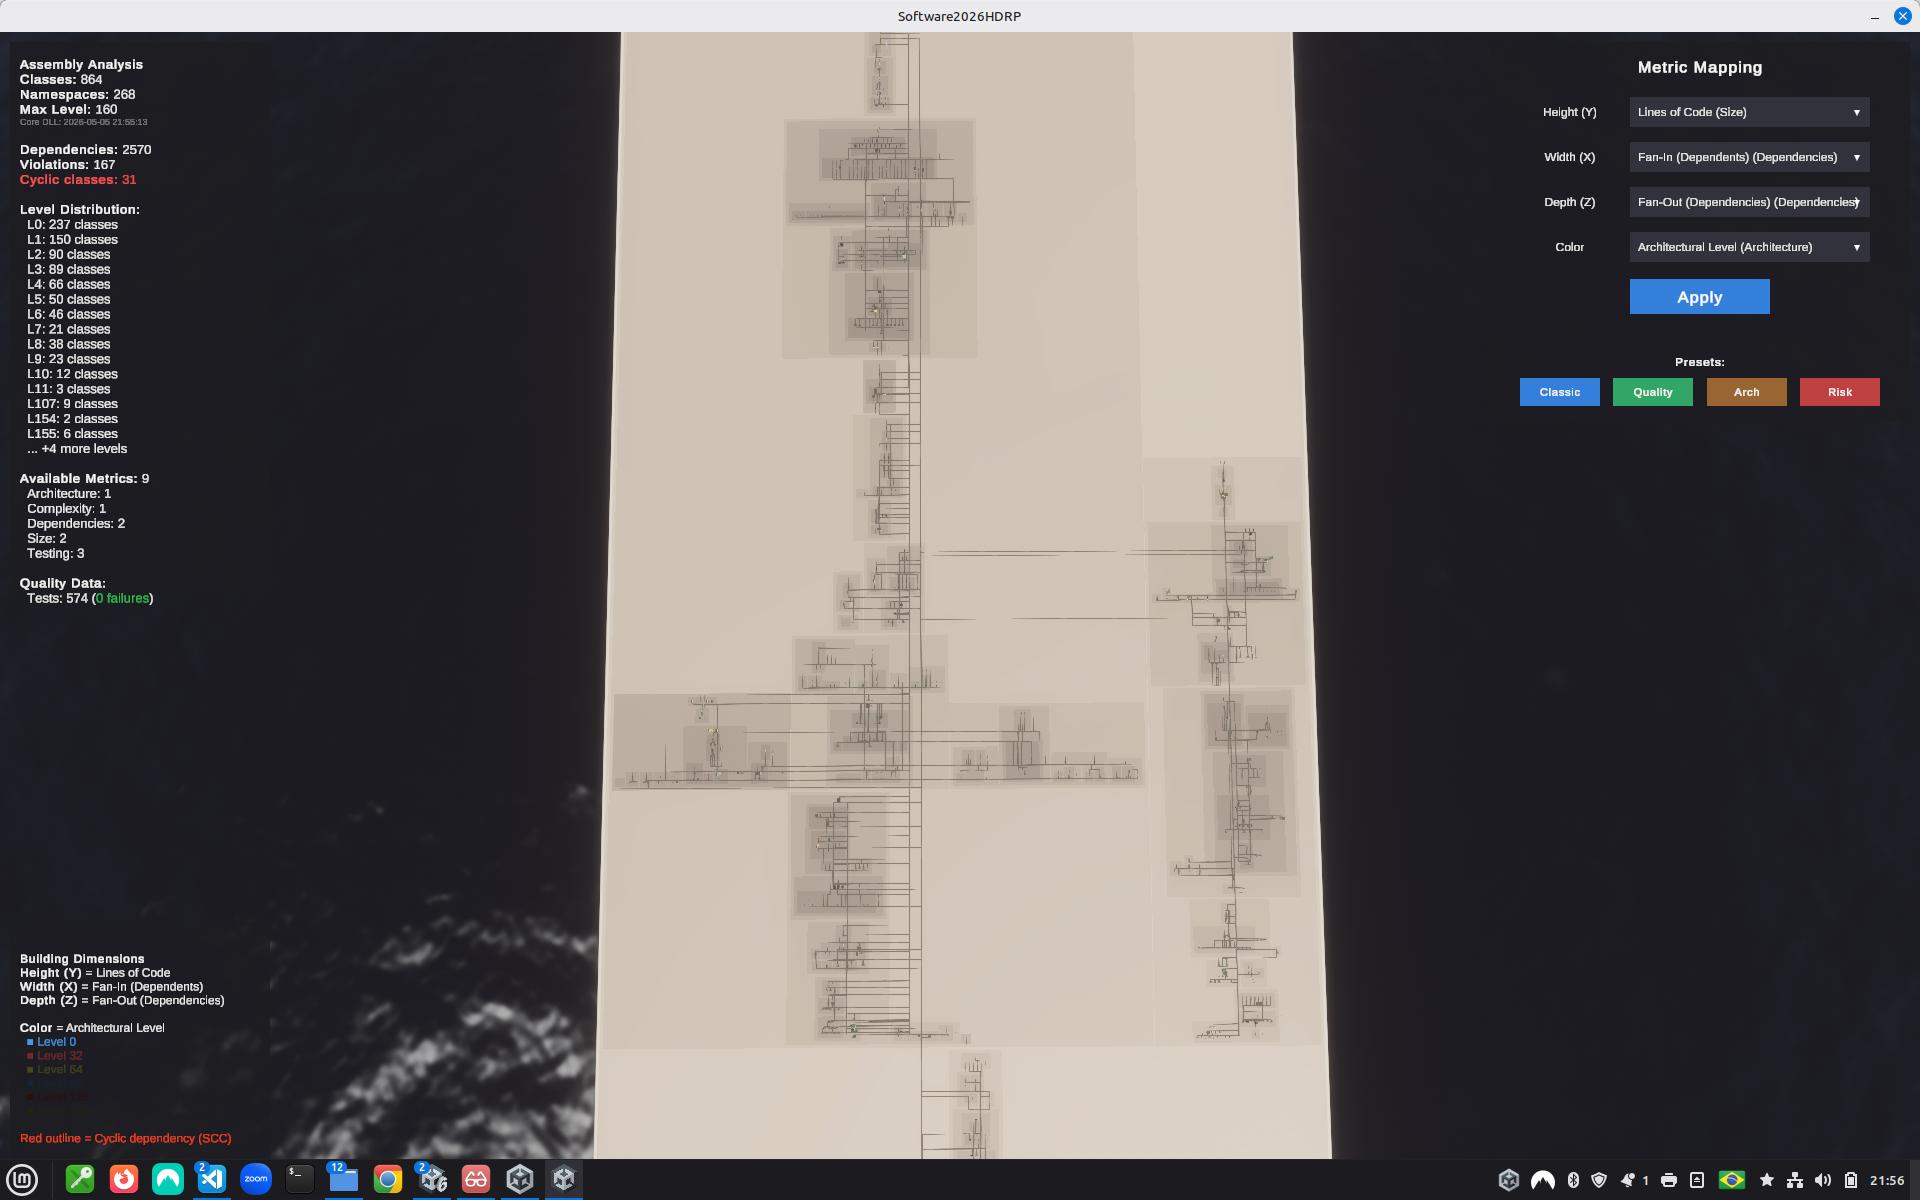
\includegraphics[width=\linewidth]{figures/SW-EKG7-Baseline.png}
    \caption{Before the fix: the full visualization looks plausible, but the
    metric panel reports 167 violations and MaxLevel 160.}
  \end{subfigure}
  \hfill
  \begin{subfigure}{0.49\textwidth}
    \centering
    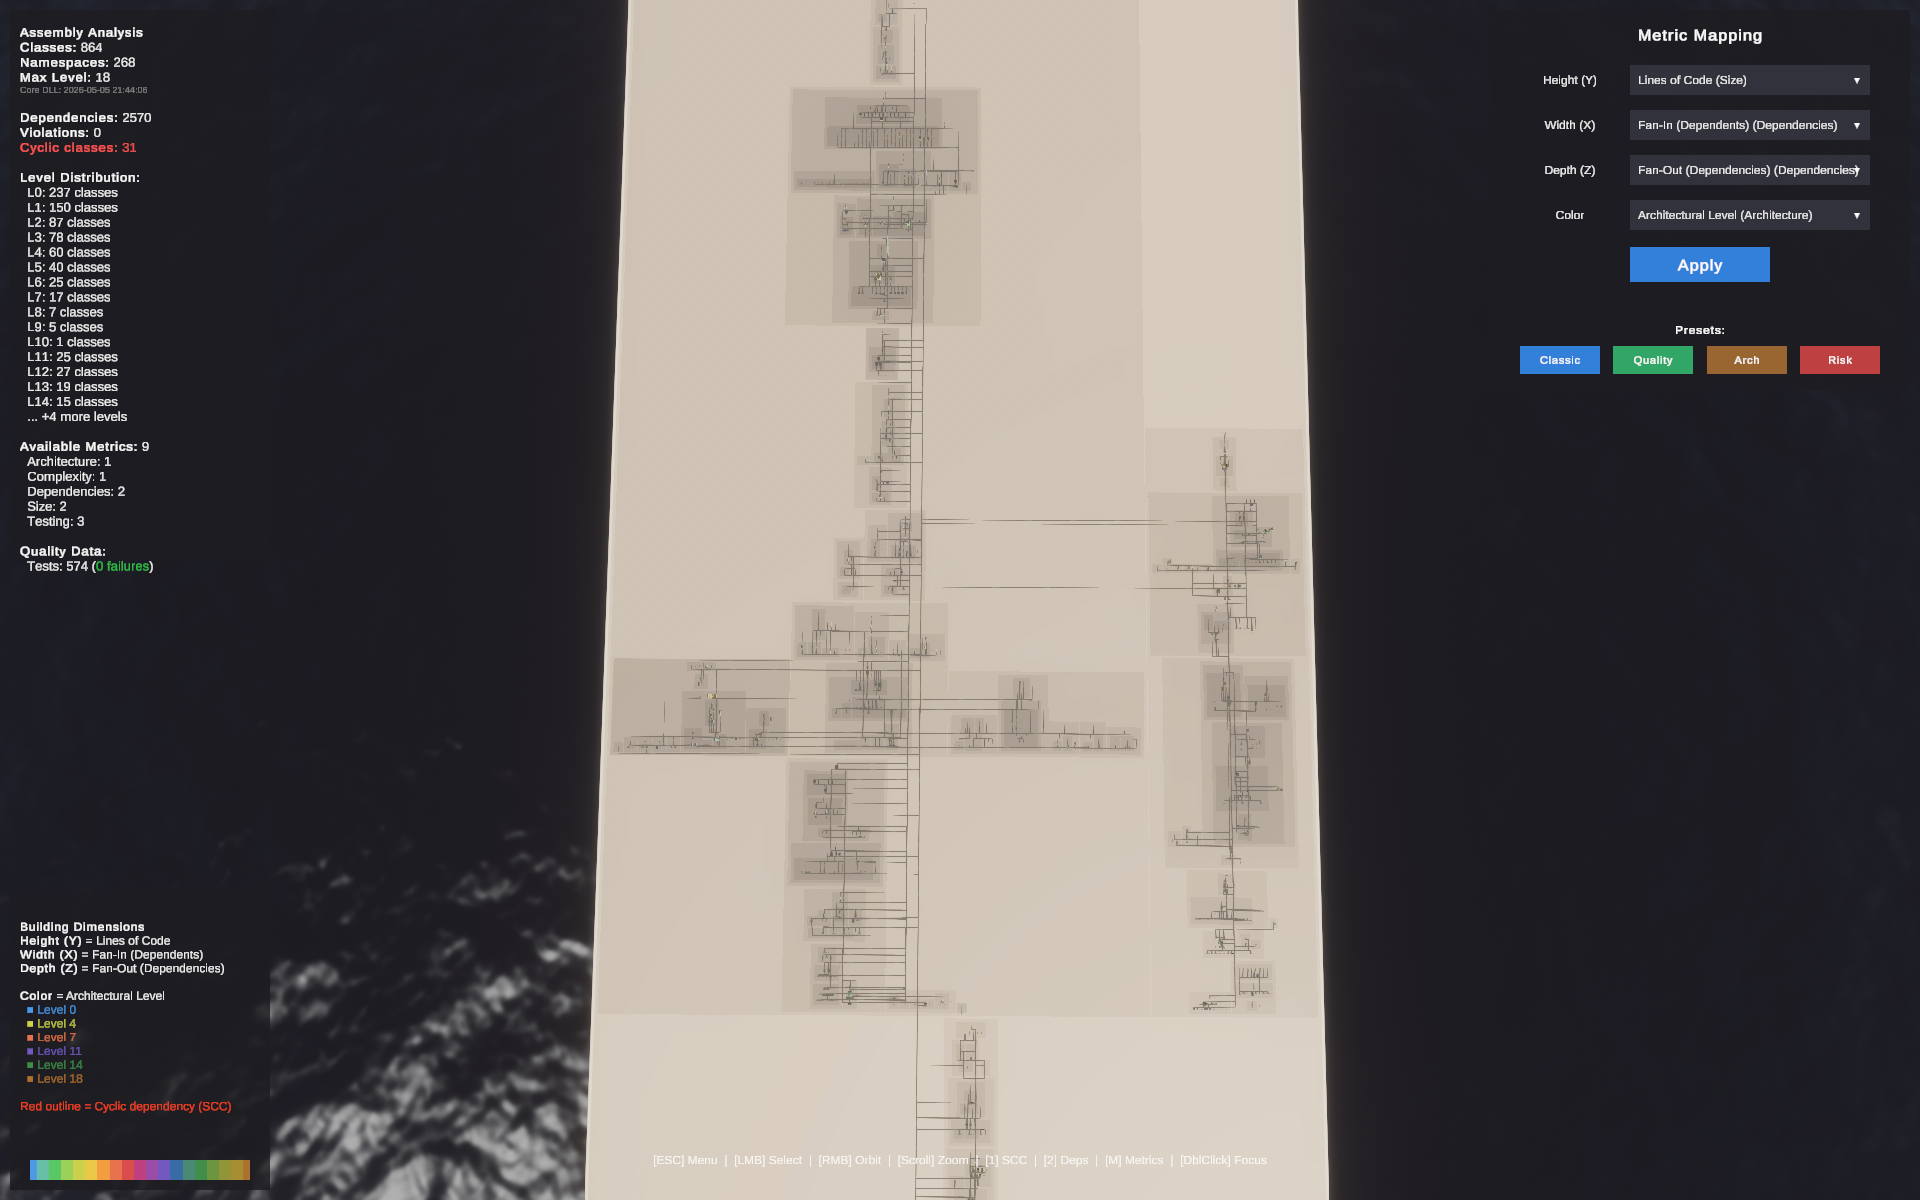
\includegraphics[width=\linewidth]{figures/SW-EKG7-Nach-Level-Fix-per-Constraint-Analyses.png}
    \caption{After the fix: the same analyzed system reports
    zero violations and MaxLevel 18.}
  \end{subfigure}
  \caption{Full-screen before/after screenshots of the \emph{software-ekg-7}
  visualization. The visible structure changes only subtly; the level metrics
  reveal the correction.}
  \label{fig:swekg7-before-after}
\end{figure}

\begin{figure}[H]
  \centering
  \begin{subfigure}{0.18\textwidth}
    \centering
    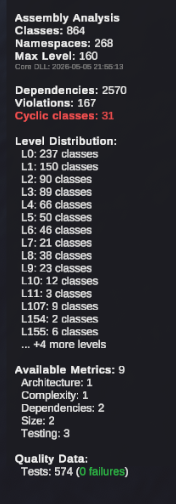
\includegraphics[width=\linewidth]{figures/Vor-Constraintfix.png}
    \caption{Before: 167 violations, MaxLevel 160.}
  \end{subfigure}
  \hspace{0.04\textwidth}
  \begin{subfigure}{0.18\textwidth}
    \centering
    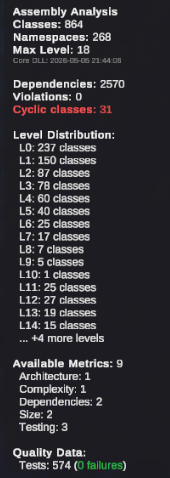
\includegraphics[width=\linewidth]{figures/Nach-Constraintfix.png}
    \caption{After: zero violations, MaxLevel 18.}
  \end{subfigure}
  \caption{Cropped metric panels from Figure~\ref{fig:swekg7-before-after}.
  These panels are the clearest user-visible symptom of the propagation
  defect and its fix.}
  \label{fig:swekg7-metrics}
\end{figure}

\subsection*{Summary}

Correct level computation for layered architecture visualizations requires
keeping three questions separate: where does a class sit in the global class
dependency stack, where does a package sit in the weighted package dependency
order, and where should an element's box go inside its parent container? Every
straightforward single-pass approach over a unified graph collapses these
questions into one coordinate, and the failure modes documented above show why
each obvious simplification breaks down in practice.

S202 resolves this by computing three values on three independent
graphs. \emph{Class architecture levels} are the longest path in the
SCC-collapsed class dependency DAG; they represent global architectural depth.
\emph{Package architecture levels} derive from a weighted inter-package
dependency graph whose edges carry aggregated method-call counts; they
represent module dependency position independently of class levels.
\emph{Local levels} come from the per-parent
sibling-only graph closed within that parent's subtree; they decide visual Y
position inside each box without disturbing either architecture coordinate.
All three use the same algorithmic shape: Tarjan SCC detection, weight-based
back-edge identification, DAG condensation, longest-path propagation.

A horizontal row-ordering pass (Phase~4) improves the legibility of dependency
overlays without modifying any computed value or affecting any layout invariant.
Five machine-checkable invariants (R1-algo, R1-visual, R2, R3, R5) run after
each analysis as implausibility alerts to the developer and emit reproducer
blocks for each finding. Four of them are pipeline-defect alerts that never
fire on a correct run; R1-visual fires only on remaining upward edges that
point to real architecture violations. They provide regression protection and
diagnostic evidence; the algorithmic contribution is the separation of the
three values themselves.

Two cases demonstrate the value of the separation. In \emph{software-ekg-7},
a plausible layered layout reported 167 dependency violations and a maximum
architectural level of 160 before a package-level equalization fix; after the
fix, the same input produced zero violations and a maximum level of 18 with
no change to the analysed source code. On Minecraft Forge~1.19.2, introducing
the local level as a distinct layout coordinate, lifting the parent
filter from the weighted package graph, and preserving the computed package
order in the UI instead of reordering it to suppress cycles, reduced the
visual upward-edge count from roughly~6\,000 to~4\,157; the eliminated edges
were artifacts of forcing parent packages below their sub-packages to keep
them out of the algorithm's tangle list, and the 4\,157 remaining edges are
real architecture violations or explicit heuristic cuts that deserve a
code-level fix.

\subsection*{Questions and Answers}

\noindent\rule{\textwidth}{0.4pt}
\vspace{0.75em}

\textbf{Why does S202 need a separate hierarchy for packages?}

Because S202 orders classes and packages by different criteria. A class level
is the depth of a node in the class dependency DAG after SCC handling: if class
$A$ depends on class $B$, then $A$ belongs above $B$ unless the edge is an
explicit heuristic back-edge or both classes remain in the same SCC.

A package level answers a different question. Packages are containers, and a
single package can contain many classes with dependencies in both directions.
S202 therefore cannot derive package order from the deepest class inside the
package. Instead, it compares the weighted relations between packages: when
the traffic from package $P_A$ to package $P_B$ dominates the reverse traffic,
$P_A$ becomes the higher dependent package and $P_B$ the lower package
it depends on. S202 keeps equal or near-equal bidirectional traffic as a cyclic
peer relationship.

This is why S202 computes class architecture levels and package architecture
levels on separate graphs. The separation prevents class depth from
accidentally lifting containers and prevents package aggregation from changing
the meaning of class-level dependency depth.

It also prevents a feedback loop. If S202 derived package levels from class
levels and then fed them back into class or layout ordering, each update could change
the input of the next update. A package moves because one contained class moves;
that package movement then changes sibling order or parent order; the changed
order can expose another cycle or another dominant relation. Sorting and
leveling algorithms then no longer operate on a stable graph. The result can
depend on traversal order, classpath order, or on how often the loop is run.
The system may converge accidentally, oscillate, or settle on a layout that is
only an artifact of the update sequence. Separating the graphs makes each phase
operate on fixed input and gives the invariants a well-defined result to check.

\textbf{Why does S202 need both an architecture level and a local UI level?}

Because these two numbers answer different questions. The architecture level
of a class says how deep the class is in the global dependency graph: how many
dependency steps separate it from the lower end of the class DAG after SCC
handling. This is a system-wide analysis value.

The local level answers a layout question: where should this class or
sub-package be placed relative to the other direct children of the same package?
That question cannot be answered reliably from the global architecture level
alone. A class can have a high global architecture level because it depends on
deep chains elsewhere in the system, even though inside its own package it is
not the highest local element. Conversely, a package-level coordinator may need
to sit above a sub-package it calls into, even if their global architecture
levels do not express that local relationship.

Using only the global DAG level for layout therefore over-constrains the
picture. Elements can be pulled too high by dependencies outside their local
container, and subsequent sorting passes try to repair a layout decision with
the wrong input value. That is hard to make stable because the global level and
the local sibling order are coupled through unrelated dependencies.

S202 keeps both values. The architecture level remains the semantic dependency
depth used for global checks and reports. The local level is recomputed
inside each package from the sibling-only graph and is used for visual ordering
inside that package. The renderer can then place elements correctly within a
container without changing what their global architecture level means.


\clearpage

\section*{Appendix B -- LevelCalculator Reference Implementation}

The following source excerpt is the complete Java implementation of the level
pipeline discussed above.

\lstinputlisting[style=appendixjava]{../../analyzer/src/main/java/de/weigend/s202/domain/architecture/LevelCalculator.java}

\vspace{1em}
The companion class \texttt{LocalLevelCalculator} implements Phase~3 (Step~6).

\lstinputlisting[style=appendixjava]{../../analyzer/src/main/java/de/weigend/s202/domain/architecture/LocalLevelCalculator.java}

\end{document}
